\chapter{Planificación}

En este capítulo se comentará la planificación inicial de tiempo en la que se llevará a cabo este TFM, la estimación en horas de cada módulo de tareas, la metodología de trabajo, los resultados y los presupuestos.

\section{Planificación temporal inicial}

La fecha de inicio trabajando en el proyecto que me fijé es el 1 de diciembre de 2016 y se espera llegar a la convocatoria de julio de 2017 por lo que se cuentan con siete meses. No obstante, y como es lógico, no voy a trabajar exclusivamente en este proyecto durante estos meses pues tengo que cursar el resto de asignaturas del máster, además debería tener un mes de margen para pulir la memoria desarrollando algunas secciones y organizando lo que haya ido apuntando durante el resto de meses. Por lo que serían 6 meses de desarrollo.

Para organizarme he decidido dedicar un número de horas semanales al desarrollo de este proyecto. Inicialmente me he fijado 15 horas a la semana dando un total de 360 horas de desarrollo puro excluyendo la redacción de la memoria.

Ordenando los módulos por prioridades y dependencias se tendría la siguiente planificación:

\begin{longtable} {l c c c}
	\hline
	\textbf{Tarea}			&	\textbf{Duración}	&	\textbf{Comienzo}	&	\textbf{Fin}	\\
	\hline \hline
	\endhead
	\hline 
	Exportación/importación	&	2 semanas			&	01/12/2016			&	14/12/2016		\\
	\hline
	Filtrado				&	6 semanas			&	15/12/2016			&	25/01/2017		\\
	\hline
	Segmentación			&	10 semanas			&	26/01/2017			&	05/04/2017		\\
	\hline
	Documentación			&	8 semanas			&	06/04/2017			&	31/05/2017		\\
	\hline
	Mejoras					&	1 semana			&	01/06/2017			&	07/06/2017		\\
	\hline
	Memoria					&	4 semanas			&	08/06/2017			&	05/07/2017		\\
	\hline
	\\
	\caption{Planificación inicial}
	\label{tab:planificacion/planificacion-inicial}
\end{longtable}

\subsection{Diagrama de Gantt}

Aunque el diagrama de Gantt tiene más sentido cuando se pueden paralelizar tareas y al haber un único desarrollador esto no es posible, realicé este diagrama porque de un vistazo se ve más clara la planificación que con la tabla anterior.

\begin{figure}[H]
	\centering
	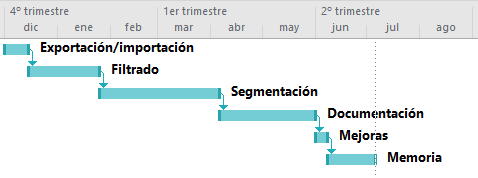
\includegraphics[width=12cm]{imagenes/planificacion/gantt}
	\caption{Diagrama de Gantt con la planficación inicial del proyecto generado con \textit{Microsoft Office Project 2016}}
	\label{fig:planificacion/gantt}
\end{figure}


\section{Metodología de trabajo}

\subsection{\textit{GitHub}}

Aprovechando que se está usando \textit{git} como sistema de control de versiones en un repositorio de \textit{GitHub}, voy a aprovechar todos los recursos que nos ofrece esta plataforma para organizarme. 

\subsection{\textit{Issues}}

En lugar de tener por un lado un tablero \textit{kanban} (por ejemplo \textit{Trello}), yo voy a utilizar los \textit{issues} (Figura \ref{fig:planificacion/issues}) de mi repositorio en \textit{GitHub} para organizar las tareas, así como ir añadiendo tareas nuevas que vaya necesitando y tener un registro de qué he hecho y cuándo, que problemas han surgido, etc.

\begin{figure}[H]
	\centering
	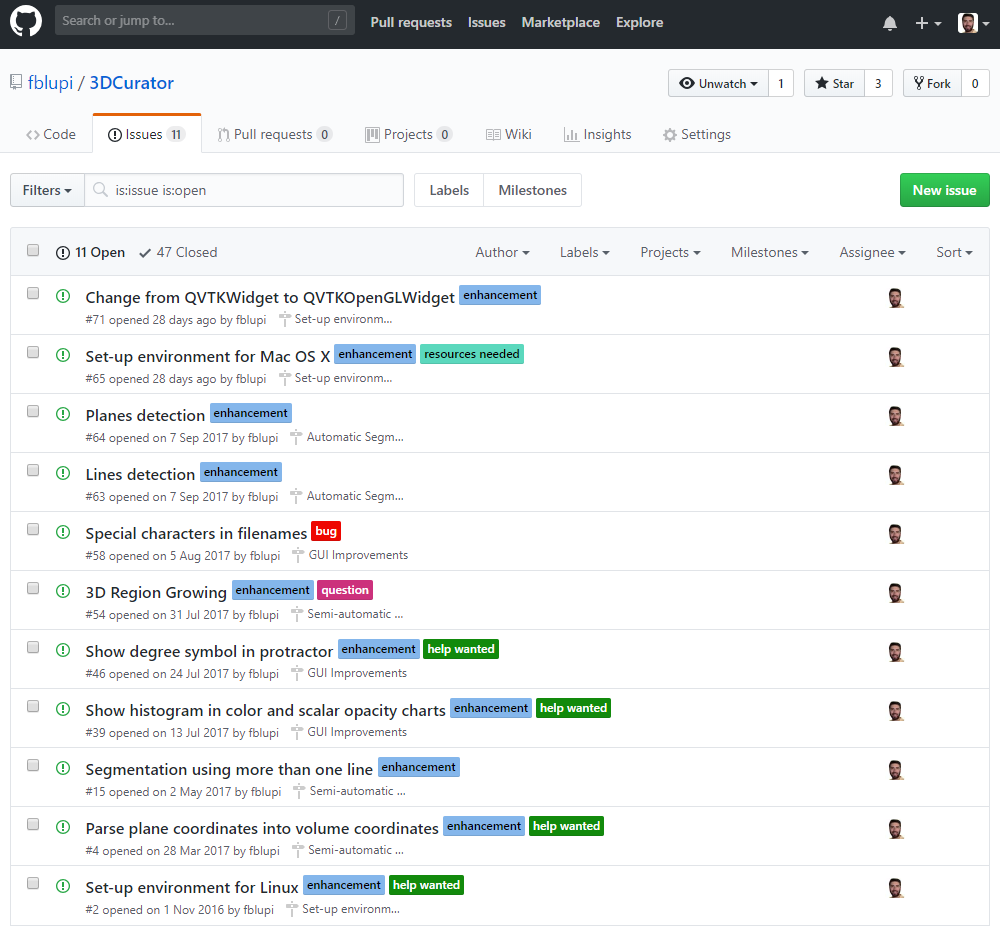
\includegraphics[width=12cm]{imagenes/planificacion/issues}
	\caption{Vista con la lista de \textit{issues} abiertos con sus correspondientes etiquetas y el \textit{milestone} al que pertenecen}
	\label{fig:planificacion/issues}
\end{figure}

Una de las ventajas de utilizar los \textit{issues} de \textit{GitHub} antes que otra plataforma como \textit{Trello} es la posibilidad de referenciarlos en los \textit{commit} agregando \texttt{\#ref} en el mensaje. Y dentro del propio \textit{issue} se vería una lista de todos los \textit{commit} donde se ha trabajado en éste. Además, si antes de escribir la referencia del \textit{issue} se añade \texttt{closes}, el \textit{issue} se cerrará automáticamente sin necesidad de hacerlo de forma manual.

\subsection{\textit{Milestones}}

Voy a clasificar los \textit{issues} por \textit{milestones} (Figura \ref{fig:planificacion/milestones}), uno por cada módulo y al mismo tiempo voy a agregarles \textit{tags} para etiquetarlos según sean \textit{bugs}, mejoras, bloqueantes por necesidad de recursos o por ayuda necesitada, etc.

\begin{figure}[H]
	\centering
	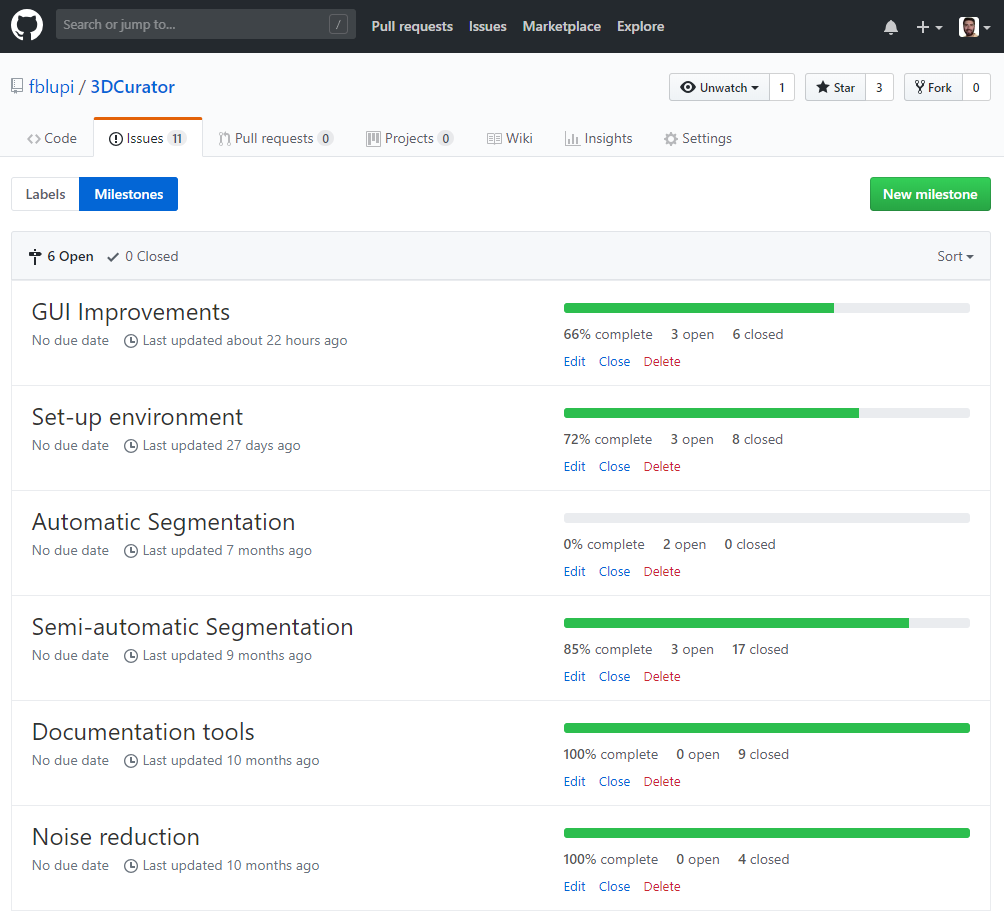
\includegraphics[width=12cm]{imagenes/planificacion/milestones}
	\caption{Resumen de los \textit{milestones} con su porcentaje de elaboración}
	\label{fig:planificacion/milestones}
\end{figure}

\subsection{\textit{Branches}}

La organización que voy a llevar en cuanto a las ramas (\textit{branches}), es la siguiente, basada en \textit{Gitflow} \cite{gitflow}:

\begin{itemize}
	\item \textbf{\textit{master}}: Esta rama tendrá la última \textit{release} del programa. Debe ser completamente estable, pues es de donde se generan los instaladores finales de la aplicación.
	\item \textbf{\textit{develop}}: Esta es la rama principal con los últimos cambios desarrollados (Figura \ref{fig:planificacion/commits}). Cuando se tiene una batería de cambios suficiente como para generar una nueva versión del \textit{software} se realizará un \textit{pull request} a \textit{master} por lo que esta rama debe ser también estable.
	\item \textbf{\textit{features}}: Estas son ramas de trabajo que no tienen por qué ser estables. Por ejemplo, si se va a agregar un filtro \textit{gaussiano} se podría crear una rama con el nombre \textit{feature/gaussian-filter} y trabajar en esta rama hasta que se validase esta nueva funcionalidad. Entonces se haría un \textit{rebase} con \textit{develop} por si ha habido algún cambio durante el transcurso de este desarrollo para resolver conflictos y finalmente un \textit{pull request} a \textit{develop} para mezclar los cambios.
\end{itemize}

Además cuento con otras ramas auxiliares que no intervienen en el flujo de desarrollo pero donde almaceno información útil.

\begin{itemize}
	\item \textbf{\textit{design}}: En esta rama se encuentran los diagramas de paquetes y clases actualizados con la versión del software en la rama \textit{develop}.
	\item \textbf{\textit{assets}}: En esta rama se almacenan recursos como logos e imágenes utilizados en la aplicación.
	\item \textbf{\textit{user-manual}}: En esta rama se encuentra el manual de usuario de la aplicación.
	\item \textbf{\textit{gh-pages}}: En esta rama se encuentra la \textit{landing page} de la aplicación. Pues \textit{GitHub} ofrece gratuitamente alojamiento para una página web estática por repositorio.
\end{itemize}

\begin{figure}[H]
	\centering
	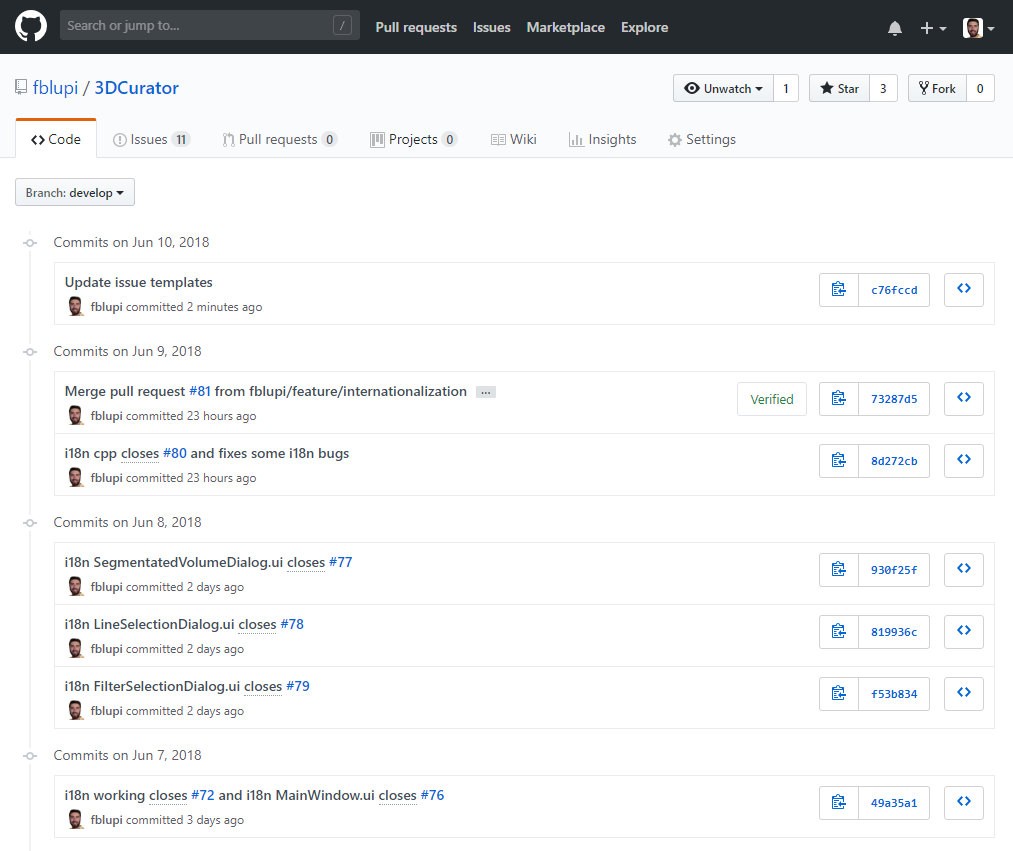
\includegraphics[width=12cm]{imagenes/planificacion/commits}
	\caption{Ejemplo de \textit{commits} en la rama \textit{develop}}
	\label{fig:planificacion/commits}
\end{figure}

\section{Resultados}

Los resultados no tienen nada que ver con la planificación inicial que se hizo. La carga del trabajo del resto de asignaturas del máster han hecho que le dedicase muchas menos horas a la semana que las que tenía pensado y durante algunos periodos lo he tenido que tener apartado.

Cuando llegó junio y vi que no llegaba a la convocatoria, recalculé tiempos para llegar a septiembre. Pero otra vez se vieron trastocados pues en agosto empecé a trabajar a jornada completa y las horas que le pude echar se volvieron a ver reducidas. No obstante llegué a tenerlo todo a excepción de la documentación. Que ya, una vez matriculado de nuevo en la asignatura la tomé con calma.

Además, me permití el lujo de añadir a última hora internacionalización al proyecto para poder tener la aplicación también en inglés además de la versión ya existente en español.

\begin{figure}[H]
	\centering
	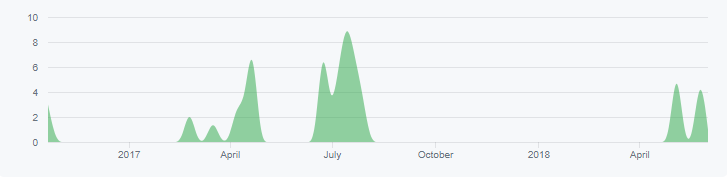
\includegraphics[width=12cm]{imagenes/planificacion/resultados}
	\caption{Gráfico de los \textit{commits} realizados en la rama \textit{develop}. El gráfico es orientativo porque hay \textit{commits} con poca funcionalidad y otros con mucha, pero ayuda a ver las etapas donde más se trabajó}
	\label{fig:planificacion/resultados}
\end{figure}

En total he registrado 312 horas de desarrollo frente a las 360 planificadas. Esto quiere decir que la planificación de tareas no ha fallado como tal. La que ha fallado ha sido la planificación de disponibilidad de recursos humanos.

\section{Presupuestos}

Este proyecto tiene costes tanto en recursos físicos como en recursos humanos. Se desglosan a continuación:

\begin{itemize}
	\item \textbf{Equipo de trabajo}: Ordenador portátil MSI CX61 2PC cuyo coste inicial es de 800 \euro{} pero tiene una vida de 4 años y al ser usado durante año y medio tendría un coste de: $ 800 \times 1.5 / 4 = 300 $
	\item \textbf{Tomografías}: El costo que tuvieron tanto la cesión como la tomografía de ambas figuras fueron de 90 \euro{} por unidad dando un total de $ 90 \times 2 = 180 $
	\item \textbf{Ingeniero informático}: El coste por hora de un ingeniero informático con mi cualificación ronda ahora mismo en el mercado laboral los 10 \euro{}/hora por lo que tendría un coste de: $ 10 \times 360 = 3600 $
	\item \textbf{Asesor}: Mi tutor hará de asesor y aproximadamente dedicará unas 36 horas entre reuniones y revisiones. Estimo unos 20 \euro{}/hora dando un total de $ 20 \times 36 = 720$
\end{itemize}

El coste total del proyecto sería de 4800 \euro{}. Se puede ver como gran parte de este presupuesto (el 92,08\%) va dedicado a recursos humanos.